\documentclass[12pt,titlepage]{article}
\usepackage[T1]{fontenc}
\usepackage[brazil]{babel}
\usepackage[utf8]{inputenc}
\usepackage{ae}
\usepackage{icomma}
\usepackage{amsmath,amsfonts,amssymb}
\usepackage{color}
\usepackage{graphicx,xr}
\usepackage{graphics}
\usepackage{tabularx}
\usepackage{booktabs}
\usepackage{times}
\usepackage{epstopdf}
\usepackage{url}
\usepackage{natbib}
\usepackage[pdftex,left=3cm,top=3cm,right=2cm, bottom=2cm]{geometry}
\usepackage{fancyhdr,epsfig,psfrag}
\usepackage{indentfirst}
\usepackage[numbib]{tocbibind} 
\renewcommand{\thetable}{\Roman{table}}
\renewcommand{\baselinestretch}{1.5} 

\begin{document}

\author{Samir Angelo Milani Martins}


\date{São João del-Rei, \today}

\title{Modelo de Relatório}
\pagestyle{fancy}

\lfoot{} \rfoot{ \hfill \small \thepage/\pageref{lastpage}} \cfoot{} \chead{}
\rhead{\small Instrumentação e Medidas - Trabalho final } \lhead{\small }

\thispagestyle{empty}

\vfill


\begin{figure}[htb] 
       	\begin{center}
       	
\includegraphics[angle=0, scale=.1]{ufsj_logo.jpg}\\       	
       	\end{center}
   \end{figure}
  
  
   \begin{center}

  \Large
  Universidade Federal de São João del-Rei - UFSJ\\
  Instrumentação e Medidas


  \vspace{3cm}

  {\LARGE Título do trabalho}

  \vspace{3cm}
  
  {\Large $\begin{array}{l c c c r}
           \mbox{Nome do aluno 1}	& & & &	\mbox{Matrícula: 0000000-0} \\
           \mbox{Nome do aluno 2}	& & & &	\mbox{Matrícula: 0000000-1} \\
          \end{array}$}
  
  \vspace{1cm}
          
  {\large \textbf{Prof:} Samir Angelo Milani Martins}
  
  
    \vspace{3cm}
 
  São João del-Rei, \today
\end{center}


\newpage

\selectlanguage{brazil}

\tableofcontents

\newpage


% ----------------------------Abstract----------------------------
\section*{Resumo}

O resumo deve vir sempre em uma página exclusiva, sem 
nenhuma outra seção. Apresentem aqui as principais ideias e os principais 
resultados do trabalho. Esta seção precisa ser bem escrita e apresentada, pois 
pode definir se o leitor irá continuar ou não a leitura. Deve conter entre 250 
e 300 palavras, não podendo em hipótese nenhuma ultrapassar uma folha. 

\newpage


% ----------------------------Introduction----------------------------
\section{Introdução}
\label{sec:intro}

Esta seção é responsável por apresentar ao leitor aspectos iniciais do tema a 
ser abordado. Apresentem o assunto de forma leve, abordando 
inicialmente aspectos mais gerais, convergindo suavemente aos itens mais 
específicos do trabalho desenvolvido.

Deve-se citar as principais referências que serviram como alicerce para o 
desenvolvimento do trabalho. Lembrem-se: ``se eu vi mais longe, foi por estar 
sobre ombros de gigantes'' (Isaac Newton).

Se optarem por utilizar o \LaTeX, os comandos \textbackslash \! cite\{\} e 
\textbackslash \! citep\{\} permitem citar referências inseridas no arquivo 
.bib. Exemplos de citação: 

\begin{enumerate}
 \item ``\cite{Martins2013} mostraram que a taxa de 
redução de erro multiobjetivo ($\cdots$)''.

 \item `` A incorporação de informação estática em modelos NARX faz com que o 
modelo seja mais adequado para esta determinada aplicação \citep{Martins2013}. 
''
\end{enumerate}


% ----------------------------Preliminaries----------------------------
\section{Conceitos Preliminares (ou Revisão de Literatura)}
\label{sec:revlit}

Esta seção é responsável por apresentar conceitos preliminares, necessários 
para o entendimento do restante do texto. Utilizem referências confiáveis, de 
modo a construir uma base sólida para a proposição do trabalho, cujos métodos 
serão detalhados na seção seguinte.



% ----------------------------Methodology----------------------------
\section{Metodologia}
\label{sec:meto}

Aqui devem ser detalhados todos os métodos utilizados para se chegar 
aos resultados obtidos. Materiais utilizados também devem ser apresentados. 
Equações matemáticas utilizadas são indispensáveis. Nenhum resultado deve ser 
apresentado nesta seção. 

Seguem exemplos de equações matemáticas no \LaTeX:

\begin{eqnarray}
f(x) &=& \int_{0}^{\infty} e^{-t}dt. \\
g(x) &=& \lim_{x \to 0} \frac{(x+5)^2}{(x+2)}. \\
h(x) &=& \frac{ \partial }{\partial x_1} (x_1^2 + x_2^2).
\end{eqnarray}



% ----------------------------Results and Discussion----------------------------
\section{Resultados e Discussões}
\label{sec:resul}

Todos os resultados devem ser apresentados aqui. Utilizem tabelas, figuras e 
texto para apresentá-los. Após a apresentação de resultados, é necessário 
discuti-los. Se preferirem, criem uma nova seção para análise e discussão.

Abaixo seguem exemplos de inserção de figuras e tabelas em \LaTeX. Para 
citá-las, utilizem comandos \textbackslash \! 
ref\{\textit{rótulo}\}. Exemplos: Figura \ref{fig:exemplo} 
e Tabela \ref{tab:exemplo}.

\begin{figure}[!hb]
  \begin{center}
    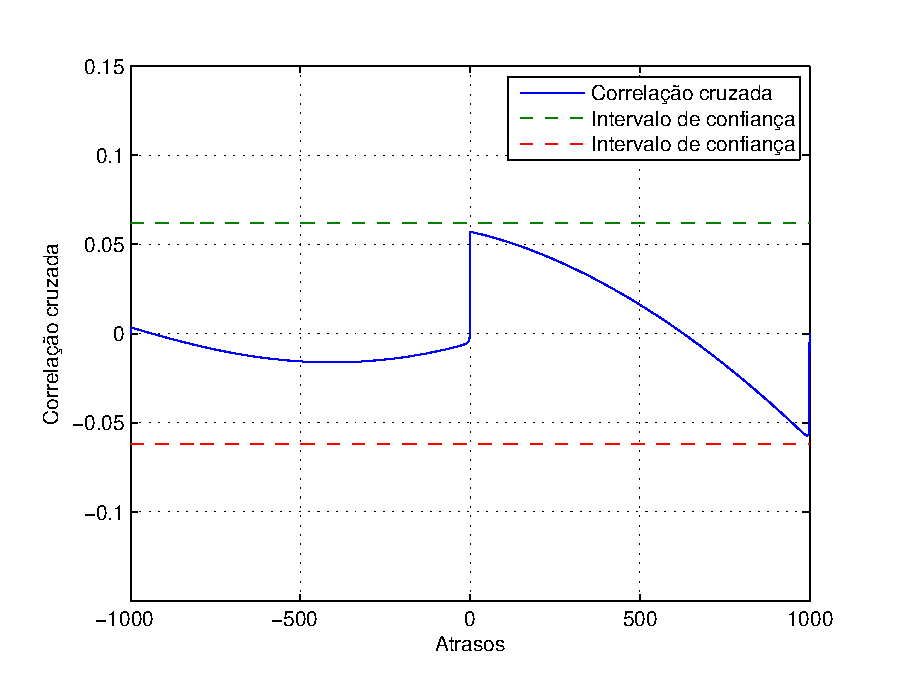
\includegraphics[scale=0.7,angle=0]{cor.eps}
  \end{center}
  \caption{Exemplo de figura.}
  \label{fig:exemplo}
\end{figure}


\begin{table}[ht]
\centering
\caption{Exemplo de tabela.}
\begin{tabular}{l l l}
\toprule
Item & Descrição & Qtde. \\
\midrule
1 & Material de consumo & 1 \\
2 & Computador (Notebook) com maleta/acessórios & 1 \\
3 & Computador (Desktop) com acessórios & 1  \\
4 & Impressora multifuncional laser & 2  \\
\midrule
 & \textbf{TOTAL} & 5  \\
\bottomrule
\end{tabular}  
\label{tab:exemplo}
\end{table}



% ----------------------------Final Remarks----------------------------
\section{Considerações Finais}
\label{sec:confin}

Nesta seção deve-se fazer uma retomada dos principais aspectos 
apresentados no trabalho, destacando as principais dificuldades 
encontradas e contribuições. Comparem o que foi proposto inicialmente 
ao que foi de fato realizado. Apresentem também propostas de melhorias para 
trabalhos futuros. Por fim, ressalta-se que nenhuma ideia nova (que não foi 
mencionada anteriormente no trabalho) deve ser apresentada aqui.

% ----------------------------Bibliography----------------------------
\bibliographystyle{apalike}
\bibliography{exemploarquivoreferencia}

% ----------------------------Appendix----------------------------
\newpage
\section*{Apêndice - Exemplo}
\label{sec:apend}

\begin{verbatim}

% Rotina Computacional Desenvolvida.
% Autores: Alunos que desenvolveram o trabalho
% Data: xx/xx/xxxx
% Versão: x.x

% Insira aqui a sua rotina

\end{verbatim}



\label{lastpage}
\end{document}

